%%%%%%%%%%%%%%%%%%%%%%%%%%%%%%%%%%%%%%%%%%%%%%%%%%%%%%%%%%%%%%%%%%%%%%%%%%%%%
\chapter{Hauptteil}
\label{chap:intro}
%%%%%%%%%%%%%%%%%%%%%%%%%%%%%%%%%%%%%%%%%%%%%%%%%%%%%%%%%%%%%%%%%%%%%%%%%%%%%
\chapterstart

\section{Theoretischer Hintergrund:}

In diesem Kapitel soll eine Basis für die Grundlegenden Technologien, Standards und Begriffe geschaffen werden, welche im Zuge der wissenschaftlichen Arbeit verglichen bzw. verwendet wurden.

Die Arbeit Untersucht die Kommunikation zwischen Frontend zu Backend Komponenten, im industriellen als auch wissenschafltichem Kontext sind diese Begriffe wie folgt definiert:

\chapquote{"Das Frontend ist das, was Ihre Benutzer sehen, und enthält visuelle Elemente wie Schaltflächen, Kontrollkästchen, Grafiken und Textnachrichten. Es ermöglicht den Benutzern, mit Ihrer Anwendung zu interagieren. Das Backend sind die Daten und die Infrastruktur, die dafür sorgen, dass Ihre Anwendung funktioniert. Es speichert und verarbeitet Anwendungsdaten für Ihre Benutzer.“}
{\cite{awsfrontendbackend}}

Wie aus dieser Definition ersichtlich beinhaltet das Front-End den benutzerspezifischen Teil und das backend den Datenverarbeitungsteil. Im Zuge der Bachelorarbeit werden anschlieden für die Front End Komponente ebenso das Wort „Client“ und für die Backend Komponente das wort „Server“ verwendet.

\subsection{Serialisierungsformate}
Bei der Übertragung zwischen der Front-End und Back-End Komponente werden Daten ausgetauscht. Da es eine Vielzahl an Technologien gibt, mit denen die jeweiligen Komponenten realisiert werden können, wurden Standards definiert, damit diese sinnvoll und effizient verarbeitet werden können.

\subsubsection{JSON}
JSON steht für JavaScript Object Notation und ist ein weit verbreitetes, textbasiertes Datenformat, das vorallem wegen einfacher Lesbarkeit und breiter Unterstützung in vielen Programmiersprachen Verwendung findet. Das Format basiert auf einer Schlüssel-Wert Paar Struktur mit einfacher Syntax ( Klammern, Spalten, Doppelpunkte, Kommas ) und kann folgende Datentypen annehmen:

\begin{itemize}
	\item String (Zeichenkette)
	\item Number (Zahl)
	\item Boolean (true/false)
	\item Array (Liste)
	\item Object (Objekt mit weiteren Schl\"ussel-Wert-Paaren)
	\item null (leerer Wert)
\end{itemize}


JSON ist der Standard für REST und GraphQL Schnittstellen.


\subsubsection{Protocol Buffers}
Protocol Buffer sind ein von Google entwickeltes Serialisierungsformat. Es handelt sich hierbei um ein binäres Serialisierungsformat, das entwickelt wurde um möglichst effizient, mit hoher Performance und mit so wenig Overhead wie möglich (ohne Whitespaces oder Satzzeichen wie bei JSON) Daten zu übertragen und zu verarbeiten. Protocul Buffer sind Plattform unabhängig und mit den meisten gängigen Programmiersprachen kompatibel.

Ein zentraler Bestandteil Protocol Buffer sind dabei plattformunabhängigen .proto Files, die für die Erzeugung definiert werden müssen.

Mit den definierten .proto Files können anschließend mit einem Plattform Abhängigen Protobuf-Compiler-Tool ( z.B. protoc ) Datenobjekte der jeweiligen Programmiersprache generiert werden.


\newpage
\textbf{\underline{Aufbau der .proto Files}}
\newline
Hauptbestandteil der .proto Files sind messages und services.

\begin{verbatim}
	message Person {
		string name = 1;
		int32 id = 2;
		string email = 3;
	}
\end{verbatim}

Messages geben dabei die Struktur der zu übertragenden Nachricht und den jeweiligen Datentypen an und einer Nummer, die beschreibt an welcher Stelle sich das jeweilige Attribut befindet, an. Die Nummerierung der Felder ist wichtig für die Serialisierung.
In Protocol Buffers können unter anderem die gängigsten Datentypen wie int32, int64, float, double, bool sowie string und bytes verwendet werden.

\begin{verbatim}
	service PersonService {
		rpc GetPerson (PersonRequest) returns (Person);
	}
\end{verbatim}

Services geben an, welche Dienste vom Server bereit gestellt werden und welche Datentypen als Parameter bei Aufruf übermittelt und als Rückgabe zurückgegeben werden. Services müssen auf der Seite des zur Verfügung stellenden Dienstes ausimplementiert werden.

Das Protobuf Serialisierungsformat wurde vorallem für die inter-server Kommunikation ( innherhalb der Backend seitigen Kommunikation) entwickelt, im Zuge der Bachelorarbeit wird diese auf die Verwendung in der Frontend zu Backend Kommunikation untersucht.

\subsection{Übertragung binärer Daten (Blob)}:
Für das Übertragen von großen binären Objekten ( wie Bilder, Video, Audiodateien, Dokumente, .. ) wird eine große Menge an binären Daten ( Datentyp: byte) gesendet. Solche großen binären Dateien, die bei der Kommunikation zwischen Client und Server gesendet werden, werden in der Webentwicklung, und vorallem im Frontend wo diese Mediendaten verarbeitet werden sollen, oft als Blob ( Binary Large Object ) bezeichnet. 


\subsection{Transportprotokolle}
Die eigentlichen Daten, die in Form von Serialisierungsformaten zwischen Frontend und backend ausgetauscht werden, werden mithilfe von Transportprotokollen von dem Client and den Server, und umgekehrt, übermittelt. Das Hypertext Transfer Protocol (http) ist dabei für moderne Webanwendungen das zentrale und verbreitetste Transportprotokoll. Im Kontext der Bachelorarbeit, wird insbesondere auf zwei Versionen von http eingegangen:

\subsubsection{HTTP/1.1}

http/1 Ist der momentan am weitesten verbreitetste Protokoll für die Kommunikation zwischen Frontend und Backend anwendungen. Es wird von allen Webbrowsern ohne einschränkungen unterstützt und bildet die Grundlage für die API Technologien REST und GraphQL. Das Protokoll funktioniert mittels eines request-responds Prinzips und überträgt die Daten über eine textbasierte Verbindung mittels eines TCP Transportprotokolls. 

\begin{figure}[htbp]
	\centering
	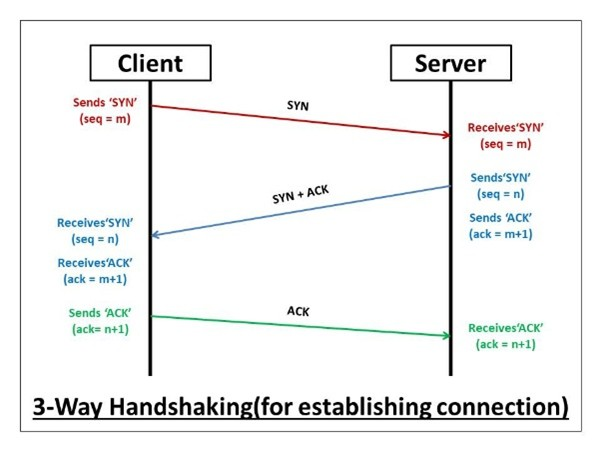
\includegraphics[width=0.7\textwidth]{images/http1_theory.jpg}
	\caption{3-Way Handshake (for establishing TCP connection)}
	\label{fig:threewayhandshake}
\end{figure}

Der Verbindungsaufbau erfolgt dabei mittels eines Transmission Control Protocol  (TCP) – Handshakes, welcher für eine zuverlässige Verbindung zwischen zwei Systemen verwenden wird. Dabei werden in drei Schritten Steuerpakete ausgetauscht:

1. Zuerst sendet der Client ein SYN (Synchronize( – Paket an den Server

2. Der Server antwortet mit einem SYN – ACK ( Acknowledge) Paket

3. Der Cient antwortet mit einem ACK

Ernst nach diesen Schritten, gilt die Verbindung als aufgebaut und die Daten werden übertragen.

Vorallem wegen der sequentielle Abarbeitung  und die Notwendigkeit von mehreren Verbindungen bei parallelen Requests führt häufig zu Performance Einschränkungen, welche vorallem bei dantenintensiven Anwendungen zu Problemen führen kann. 


\subsubsection{HTTP/2}
Aufgrund der ber http/1 genannten Performance Problemen wurde eine neue Version namens http/2 Enwickelt, weche viele Schwächen von http/1.1, insbesondere beszogen auf Latenz und Effizienz, ausgleicht.
Das Hauptmerkmal von http/2 ist Multiplexing, hierbei ist es möglich mehrere parallele Anfragen und Antworten über nur eine einzige TCP-Verbindung durchzuführen.
Weitere Verbesserungen beinhalten zum Beispiel die Komprimierung von Header-Informationen oder das Server Push-Verfahren, das eine proaktive Übertragung vom Server an den Client erlaubt.
Aufgrund der oben genannten Verbesserungen wird http/2 besonders in modernen Anwendungen in denen eine schnelle und effiziente Datenübertragung wichtig ist, wie biespielsweise bei gRPC, Echtzeitkommunikation oder Microservices verwendet.
Webbrowser unterstützen nur eine eingeschränkte Nutzung von http/2 deshalb können bei der Kommunikation zwischen Webbrowsern und Serveranwendungen nicht alle Vorteile ausgenutzt werden. Zwar unterstützen aktuelle Webbrowser mittlerweile http/2, jedoch ist bei der verwendung eine verschlüsselte Übertragung verpflichtend, und wichtige Features wie echted bidirektionales Streaming (gleichzeitiges Senden und Empfangen von Daten durch Client und Server) oder http/2 Trailers (das Übermitteln zusätzlicher Metadaten am Ende einer Übertragung, z.B. zur Fehlerbehandlung, welche bei gRPC zum einsatz kommen, werden in Webbrowsern nicht bzw. nur teilweise unterstützt. Dadurch können bei der Kommunikation zwischen Frontend (Webbrowser) und Backend nicht alle Potenziale von HTTP/2 ausgeschöpft werden 


\subsection{API-Technologien}
Eine API ist eine Schnittstelle eines Softwaremoduls, welche es ermöglicht, dass das jeweilige Softwaresystem mit einem anderem System kommunizieren kann.
Eine Web API sind APIs die von Web-Servern zur Verfügung gestellt werden. Bei webservern findet die Kommunikation mit einem der http bzw. https Protokollen statt. Da sich die Forschungsfragen und der Prototyp gezielt auf die Kommunikation zwischen einem Web Frontend und einem Webserver beziehen, bezieht sich der Begriff API im folgenden immer auf Web APIs.

API Technologien wie REST, GraphQL oder gRPC legen Standards fest ( Konventionen, Art der Serialisierungsobjekte, Art des Transportprotokolls) die neben der technischen Kompatibilität für die Kommunikation auch Entwicklern hilft, sich effizient in API-Systemen zurecht zu finden.


\subsubsection{Representational State Transfer (REST)}

Der REST-Architekturstuk wure im Jahr 1994 von Roy Fielding im Rahmen seiner Dissertation entwickelt, mit dem Ziel eine bis dato einfache Alternative für die Kommunikation zwischen zwei Systemen zu schaffen. 

\textbf{\underline{Infrastruktur:}}
Eine API-Schnittstellt ist nach Definition nur dann im REST Stil umgesetzt, falls folgende 5 Eigenschaften erfüllt werden:


\begin{itemize}
	\item \textbf{Client-Server:}
	Das System muss sich in einer Server-Client Architektur umgesetzt werden. Besteht aus einem Server, der einen Dienst oder Daten bereitstellt und einem Client, welcher diese Dienste nutzen kann. Server und Client kommunizieren mittels Nachrichten, indem mittel eines Request-Respond Prinzips der Client eine Anfrage (Request) schickt und der Server eine Antwort (Respond)
	zurückliefert.
	
	\item \textbf{Zustandslosigkeit:} 
	In jeder Nachricht, die zwischen Server-Client verschickt werden müssen alle Informationen enthalten sein, damit der jeweilige Kommunikationspartner die Nachricht verarbeiten kann. Es ist nicht erlaubt Zustandsinformationen zwischen zwei Nachrichten zu speichern.
	\item \textbf{Caching:}
	HTTP Caching soll benutzt werden, hierbei werden Daten in einem Cache gespeichert und bei nochmaligem abfragen vom Cache abgefragt, um unnötige Serveranfragen und Datenübertragungen zu vermeiden.
	\item \textbf{Einheitliche Schnittstelle:}
	Eine einheitliche Schnittstelle ist wie folgt definiert:
	
	\begin{enumerate}
		\item \textbf{Addressierbarkeit von Ressourcen:}
		Jede Ressource im System ist eindeutig über eine URI adressierbar.
		\item \textbf{Repräsentationen zur Veränderung von Ressourcen:}
		Ressourcen können durch verschiedene Formate (wie JSON oder XML) repräsentiert und über Standard-HTTP-Methoden verändert werden.
		
		\item \textbf{Selbsbeschreibende Nachrichten:}
		Jede Nachricht enthält alle notwendigen Informationen, damit der Empfänger sie interpretieren und verarbeiten kann.
		
		\item \textbf{„Hypermedia as the Engine of Application State“ (HATEOAS):} 
		Bei HATEOAS stellt der Server dem Client Links zur Verfügung, mittels dem der Client auf weitere Ressourcen zugreifen kann.
	\end{enumerate}
	
	\item \textbf{Mehrschichtige Systeme:}
	Systeme sollen mehrschichtig aufgebaut sein, die Kommunikationsparner müssen aber jeweils immer nur die oberste Schicht kennen.
	
	\item \textbf{Code on Demand (optional):}
	Im Bedarfsfall kann der Server dem Client Code zur Verfügung stellen. Diese Eigenschaft ist für einen REST Architekturstil jedoch nur optional.
\end{itemize}

Viele Web Dienste, erfüllen bereits viele dieser Eigenschaften wodurch sich REST zu einem beliebten Standard entwickelt hat.

\textbf{\underline{Kommunikation zwischen Client – Server:}}
Die Kommunikation zwischen dem findet bei REST fast ausschließlich über http/HTTPs statt, wobei laut Definition kein spezifisches Transportprotokoll vorgeschrieben wird. Im Zuge der Arbeit und der weiten Verbreitung wird im Zuge der Arbeit ausschließlich http verwendet.

HTTP stellt für den Zugriff auf Ressourcen eine Reihe an Methoden zur Verfügung. Die wichtigsen http Methoden sind : \newline

\begin{tabularx}{\textwidth}{|l|X|}
	\hline
	\textbf{HTTP Methode} & \textbf{Beschreibung} \\
	\hline
	GET & GET fordert eine Ressource vom Server an. Der Zustand des Dienstes bzw.\ der Ressource wird dabei nicht verändert. \\
	\hline
	POST & Fügt in den meisten Fällen eine neue Ressource ein. Kann aber auch verwendet werden, um Methoden zu realisieren, die durch keine andere HTTP-Methode abgedeckt werden. Ändert den Zustand des Servers. \\
	\hline
	UPDATE & Ändert den Zustand einer bestehenden Ressource. \\
	\hline
	DELETE & Löscht eine bestehende Ressource. \\
	\hline
\end{tabularx} \newline


Der Zugriff auf die Resourcen erfolgt bei REST jeweils über die URL.

\clearpage
\subsubsection{GraphQL}
GraphQL ist eine open source Datenabfrage- und Manipulationssprache und wurde im Jahr 2015 von Facebook veröffentlicht.
Der Standard wurde entwickelt, um eine bessere Alternative für REST Architekturen und SQL bereitzustellen, da bei REST Anwendungen eine vordefinierte Satz von Daten an den Client  zurückgeliefert wird. Vor allem bei mobilen Anwendungen führte diese Einschänkung zu Problemen, da oft zu viele bzw. zu wenig Daten übermittelt wurden, was zu einem unnötigen Übertragungsvolumen führte.
GraphQL erlaubt es dem Client gezielt die benötigten Daten abzufragen. Außerdem können Daten, welche in mehreren Datenobjekten verschachtelt sind, effizient abgebildet werden. Diese Eigenschaften machen GraphQL im Kontext der Datenabfrage besonders effizient und flexibel, da somit keine unnöige Datenübertragung stattfindet. 


\subsection*{Unterstützte Operationen}

\begin{description}[leftmargin=2cm, style=nextline]
	\item[Queries (schreibend):]  
	Queries definieren die exakten Daten die vom Client angefordert werden. Die Daten werden in der selben Struktur an den Client zurückgesendet.
	
	\item[Mutations (manipulierend): ]  
	Mit Mutations können Daten manipuliert werden, ähnlich wie POST, UPDATE oder DELETE Funktionen bei REST. Mutations beinhalten Variablen welche vom GraphQL Server verarbeitet werden und die Struktur, welche die Struktur für den Response definiert.
	
	\item[Subscriptions:]  
	Erlauben Live Updates von dem Server an den Client. Die Struktur gibt die Struktur der Nachrichten an welche an den Client übermittelt werden. 
\end{description}

\subsection*{Technische Umsetzung}

Technische weden GraphQL Requests und responses in einem JSON Format übertragen und die Kommunikation findet über das http Protokoll statt. Außerdem is es Konvention, dass typisherweise alle Operationen (Queries, Mutations, Subscriptions) über einen einzigen Endpunkt (/graphql) laufen.
Die Anfrage wird dabei als String im sogenannten „GraphQL Query Language“-Format an den Server geschickt. Die Antwort enthält die angeforderten Daten innerhalb eines „data“ Feldes und im Fehlerfall ein „error Feld“ in dem die jeweiligen Fehler und Details angeführt werden.

\clearpage
\subsubsection{Google Remote Procedure Calls (gRPC)}
gRPC ist ein im Jahr 2015 veröffentliches open-source Framework mit dem Remote Procedure Calls (RPC) durchgeführt werden können. Die Grundidee von gRPC geht darauf zurück, dass Google eine modernes und performante Technologie entwickeln wollte, das auf einem bereits intern eingesetztem RPC Framework names Stubby basiert. 
Stubby wurde ursprünglich innerhalb von Google entwickelt und eingesetzt, um die Kommunikation zwischen einer Vielzahl an Microservices in unterschiedlichen verteilten Systemen effizient umzusetzen. gRPC knüpft an dieser Technologie an und wurde, als Open-Source Nachfolger von Stubby veröffentlicht, um eine performante und sprachübergreifende Lösung für die Interprozesskommunikation bereitzustellen.

\textbf{\underline{Remote Procedure Call:}}
RPC beschreibt ein Kommunikationsmodell, bei dem ein Programm auf einem anderen Computer ( meist Server ) eine Methode auf einem anderen entfernten System aufruft, als wäre sie lokal vorhanden. Im Unterschied zu REST oder GraphQL sind RPC Calls Methoden (Methodenname, Parameter und Rückgabewert) und nicht Ressourcen orientiert, wodurch die Schnittstelle stärker an der Logik der Anwendung angelehnt ist. 

Hauptanwendung findet gRPC in der Kommunikation von Micro Service Architekturen und in der inter-backend-Kommunikation. Micro Services sind kleine, eigenständigen Dienste, die jeweils eine klar abgegrenzte Aufgabe erfüllen und unabhängig voneinander entwickelt werden, jedoch (häufig in hoher Frequenz und mit großen Datenmengen)miteinander kommunizieren. Hier ist es wichtig, dass die Daten performant zwischen den verschiedenen Services hin und her geschickt werden. gRPC kann jedoch auch für die Kommunikation zwischen Browsern bzw. Mobilgeräten und Backend Services genutzt werden.

Die Kommunikation von gRPC findet standardmäßig über http/2 Protokoll statt, wodurch die in http/2 eingeführten Features die zu besserer performance und effizienz führen genutzt werden können. Außerdem wird für die Serialisierung  das in 1.1.1 beschriebe Protobuff Format verwendet, welches durch die binäre Struktur zu einer weiteren Verbesserung der Performance und Effizienz führt.

\subsection{gRPC Web}
Obwohl gRPC ursprünglich für die interprozesskommunikation in Micro Services entwickelt wurde, ist es auch möglich gRPC mit Einschränkungen für die Kommunikation zwischen Web-Browsern und Backend Services zu verwenden.
Da in Web Browsern nicht alle Funktionen von http/2 zur Verfügung stehen kann für die Kommunikation in diesem Szenario nicht gRPC direkt verwendet werden. Für diesen Andwendungsfall wurde ein eigenes Protokoll namens gRPC-Web konzipiert. 

Folgende Funktionen von gRPC stehen dadurch nicht zu Verfügung:
bidirektionales streaming (Full Duplex Streaming), Volle Kontrolle über HTTP/2-Funktionen (z.B. Header-Komprimierung, Multiplexing, Flow-Control), gRPC-Reflection
Folgende Eigeschaften bleiben bei der Verwendung des gRPC-Web Protokolls erhalten:
Protobuf als effizientes Datenformat, , Codegenerieung für Server und Client, Typensicherheit, Contract-first Api mit .proto Dateien, Server-Side Streaming

Oft wird gRPC-Web über einen Proxy ( z.B Envoy oder gRPC-Web-Proxy) an einen regulären gRPC-Server weitergeleitet. Dies muss gemacht werden, da gRPC-Web zwar http/1.1 oder eingeschränktes http/2 (wie es im Browser verfügbar ist) verwendet, der eigentliche gRPC Server jedoch auf vollem http/2 basiert. Ein solcher Proxy übernimmt die „Übersetzung“ zwischen gRPC-Web und grpC (Backend). Für diese Übersetzung gibt es verschiedene gängige Varianten:

\begin{enumerate}
	\item \textbf{Envoy Proxy:}
	Envoy ist ein moderner Proxy, der nativ gRPC-Web unterstützt. Er führt die „Übersetzung“ druch und leitet sie intern an den gRPC-Server weiter.
	→ Vorteil: Skalierbar, performant
	→ Nachteil: Zusätzlicher Deployment-Aufwand (eigene Proxy-Instanz)
	
	\item \textbf{gRPC-Web-Proxy :}
	Ein Node.js-basierter Proxy, der ebenfalls als Brücke zwischen Browser und gRPC-Backend dient.
	→ Vorteil: Schnell einzurichten
	→ Nachteil: Weniger leistungsfähig als Envoy
	
	\item \textbf{Direkte Serverintegration in ASP.NET Core}
	→ Vorteil: Einfaches Setup, kein Proxy nötig, ideal für .NET-Umgebungen
	→ Nachteil: weniger flexibel für komplexe Architekturen
\end{enumerate}

Im Rahmen des implementierten Prototyps für diese Arbeit wurde die direkte Serverintegration in ASP.NET Core gewählt.

Da es in der Arbeit um die Kommunikation zwischen Web Browsern und Backend Services geht, wird in folgendem nur vorallem ein Fokus auf das gRPC Web Protokoll gelegt.

\clearpage
\subsection{Begriffe}
\subsubsection{Latenz}
Der Begriff Latenz bezieht sich im Rahmen der Bachelorarbeit auf die Zeit für die übermittlung der Daten von dem Server an den Client, ab dem Senden des Requests von dem Client.
\subsubsection{Durchschnitt und Median}
Zur Auswertung von Messergebnissen wurden zwei Lageparameter verwendet: der Durchschnitt (arithmetische Mittel) und der Median. 

Der Durchcshnitt ergibt sich aus der Summe aller gemessenen Werten, dividiert durch die Anzahl der Messungen:
\[
\bar{x} = \frac{1}{n} \sum_{i=1}^n x_i
\]

Der Median bezeichnet jedenen Wert, er in einer sortzierten Messreige genau in der Mitte liegt. Er teilt die Messwerte in zwei gleich große Hälften und ist dadruch robuster gegenüber Ausreißern.

\clearpage
\subsection{Theoretische Analyse und Vergleich der API-Technologien:}

Aufbauend auf den theoretischen Grundlagen, sollen anschließend die ausgewählten API-Technologien: REST, GraphQl, gRPC und gRPC-Web direkt miteinander verglichen werden. Neben der technischen Eigenschaften sollen auch Aspekte wie Verbreitung im Frontend, Erlernbarkeit und Effizienz betrachtet werden. Ergänzend soll auch der momentane Stand der Technik eingeordnet und ähnliche wissenschaftliche Arbeiten herangezogen werden.
Ziel des Kapitels ist es, die jeweiligen Stärken und Schwächen der Technologien herauszuarbeiten und aufzuzeigen.


\section{Vor- und Nachteile der API-Technologien}

Das folgende Kapitel soll die Vor- und Nachteile der APIs aufzeigen.

\subsubsection{REST}

\paragraph{Vorteile:}
\begin{itemize}
	\item REST ist der etablierteste API-Standard für Web-APIs.
	\item Es ist im Vergleich einfach und intuitiv aufgebaut.
	\item Ein Großteil der Entwickler ist bereits mit dem Standard vertraut.
	\item Wird in den meisten Web-Clients nativ unterstützt und liefert typischerweise JSON, welches für Menschen leicht lesbar ist.
	\item HTTP-Funktionen wie Caching und Authentifizierung können direkt genutzt werden.
	\item Durch die weite Verbreitung gibt es eine Vielzahl an Tools für die Entwicklung und das Testing (z.B. Postman, Swagger).
\end{itemize}

\paragraph{Nachteile:}
\begin{itemize}
	\item Der größte Nachteil von REST ist das Over-Fetching bzw. Under-Fetching. Es gibt klar definierte Endpunkte die eine gewissen Datenansatz zurückliefern. Hierbei kann es zu dem Problem kommen, dass man mehr Daten übertragen muss, als man benötigt, was zu zusätzlichen Netzwerklast und höheren Latenzen führt.
	\item Jeder Request ist stateless, das heißt, alle Kontextinformationen müssen immer mitgeliefert werden, was bei einer Vielzahl von Requests ineffizient sein kann.
	\item Versionierung: Änderungen der API erfordern oft neue Endpunktversionen, was die Wartung erschweren kann.
	\item Auch wenn meist JSON für die Übertragung genutzt wird, gibt es an sich keine strikte Typsicherheit. 
\end{itemize}

\subsubsection{GraphQL}

\paragraph{Vorteile:}
\begin{itemize}
	\item GraphQL bietet eine präzise Datenabfrage, der Client bekommt genau die Menge an Daten, die benötigt wird, Over-Fetching bzw. Under-Fetching wird verhindert.
	\item Mehrere Ressourcen können in einer Anfrage kombiniert werden, im Gegensatz zu REST, wo mehrere Endpunkte separat aufgerufen werden müssen. Diese Eigenschaft verringert die Netzwerkrundläufe, was vor allem bei langsamen oder mobilen Verbindungen effizient ist.
	\item . GraphQl ist stark typisiert, alle verfügbaren Datenytpen und Felder sind definiert und können vom Client abgefragt werden, was die Entwicklung erleichtert. 
	\item Neue Felder können einfach hinzugefügt werden ohne bestehende Queries verändern zu müssen.
\end{itemize}

\paragraph{Nachteile:}
\begin{itemize}
	\item Die Flexibilität die durch GraphQl für das Frontend schafft, verlagert die Komplexität auf den Server. 
	\item Die Implementierung kann ohne Batch-Loading oder Caching-Strategien zu Performance Einbußen führen, da meistens alle Abfragen über nur einen einzigen /graphql-Endpoint per POST laufen, und somit das übliche http-Caching- nicht automatisch funktioniert. 
	\item Das fehlen des eingebauten HTTP-Caching führt dazu, dass Entwickler eigeine Cashing-Lösungen implementieren müssen. 
	\item Durch die frei gestaltbaren Queries ist es außerdem schwierig, paschale Limits oder Vorhersagen über Lasten zu definieren.
	\item Im Gegensatz zu REST ist GraphQl nicht weniger verbreitet und es gibt eine begrenztere Anzahl an Debugging Möglichkeiten.
\end{itemize}

\subsubsection{gRPC}

\paragraph{Vorteile:}
\begin{itemize}
	\item gRPC ist auch Hochleistung ausgelegt. In der Web-Variabte gRPC-Web können diese Vorteile zum Teil auch im Browser genutzt werden. 
	\item Durch das Verwenden von Protocol Buffers, sind die gesendeten Nachrichten binär kodiert, äußerst kompakt und dadurch schneller übertragen als z.B. JSON. 
	\item . In Kombination mit http/2.0 als Transport ermöglicht dies eine sehr niedrige Latenz und effiziente Ausnutzung der Verbindung (Multiplexing). 
	\item gRPC ist streng typisiert, und die zu sendenden Datenstrukturen als auch zur Verfügung stehenden Dienste sind in einer .proto Definition klar definiert. 
	\item . Dieser klare Vertrag zwischen Client und Server erhöht die Typsicherheit, reduziert messstände und Fehler zur Laufzeit.
	\item Außerdem unterstützt gRPC Streaming in beide Richtungen. 
\end{itemize}

\paragraph{Nachteile:}
\begin{itemize}
	\item Da gRPC auf http/2 basiert und davon spezielle Features nutzt, die von vielen Webbrowsern nicht unterstützt werden, ist es ohne Weiteres nicht in Browser Umgebungen nutzbar. 
	\item Die Lösung hierfür ist die Übersetzung von gRPC zu gRPC-Web, welches im Browser benutzt werden kann. Diese Notwendige Zwischenschicht erhöht jedoch die Infrastruktur-Komplexität und kann zu Fehlerquellen führen.
	\item Einige Features, die zu einer Latenzreduzierung führen, gehen dadurch verloren.
	\item gRPC wird nicht so häufig für die Kommunikation zwischen Web und Backend benutzt, dadurch gibt es weniger Debugging-Tools.
	\item Die Nutzung von gRPC ist nicht so intuitiv und einfach wie REST und erfordert eine Einarbeitung in neue Tools und Konzepte.
	\item Gerade im Frontend-zu-Backend-Kontext muss abgewogen werden, ob der Performancegewinn die erhöhte Komplexität rechtfertigt.
\end{itemize}

\subsection{Effizienzvergleich: Latenz, Datenvolumen und Ressourcenverbrauch}

\paragraph{Latenz und Antwortzeit:}  
Latenz und Antwortzeit: Durch das binäre Protokoll und http/2.0-Multiplexing sind gRPC-Aufrufe in der Regel sehr schnell in der Übertragung und haben somit die geringste Latenz. Auch in empirischen Daten wird aufgezeigt, dass gRPC die geringsten Antwortzeiten hat, gefolgt von REST. GraphQl hat dabei tendenziell die langsamsten antworten. In der Studie wurde dabei in einer Microservice-Umgebung 100-500 Datenrequests abgerufen und die Zresponse-Zeiten ermittelt. Festzuhalten ist dabei, dass es sich in der Studie um gRPC und nicht um gRPC Web handelte. Während die Antwortzeit bei GraphQl am langsamsen war, konnten hier jedoch für Anfragen mit vielen verknüpften Daten die Anzahl der benötigten http-Requests reduziert werden. Sobei war teilweise in Summe GraphQl schneller, da diese Anfrage schneller abgeschlossen war als die Summe an mehreren REST-Aufrufen. Im Gegensatz dazu, kann REST jedoch bei wiederholten Aufrufen von http-Caching profitieren.

\paragraph{Datenvolumen:}  
Für die Übertragung von sehr kleinen Payloads ( z.B. Text, JSON ) hat gRPC durch die http/2, binäre Protobuf-Serialisierung und Header-Kompression die gerngste Latenz und den niedrigsten Overhead. REST und GraphQL haben bei einfachen Einzel-Abfragen eine vergleichbare Latenzm wobei GraphQl den Vorteil hat, dass mehrere kleine Abfragen gut kombiniert werden können, wodurch Over-Fetching verhindert wird.
Auch bei großen Datenmengen (z.B. Bilder, Videos) ist gRPC durch die native Streaming Unterstützung und das binäre Framing effizienter als die anderen Technologien. REST kann große Dateien als Blob senden, dies ist aber weniger performant. GraphQl ist beim senden großer binärer Daten am wenigsten geeignet, da diese meist zuerst in base64 kodiert werden müssen, wodurch sich der Overhead um ca. 33 \% erhöht. 


\paragraph{CPU- und Ressourcenverbrauch:}  
Neben dem Senden der Nachricht über das Netzwerk müssen die Nachrichten nach dem erhalten Responses auch weiterverarbeitet werden, damit das jeweilige System mit den Daten arbeiten kann. Das Serialisieren / Deserialiseren von Nachrichtenist bei gRPC sehr effizient. Das Parsen der binären Protobuf Daten nimmt im Vergleich zu der Verarbeitung von JSON-Strings bei REST /GraphQl sehr wenig CPU-Zeit in Anspruch. Dies spart sowohl Server- als auch Clientseitig Zeit ein. Da die bei GraphQl flexibel Queries erst ausgewertet und zusammengestellt werden müssen,  ergibt sich bei dieser Technologie eine weitere Komponente die CPU-intensiv sein könnte. Auch aktuelle Untersuchungen zeigen, dass GraphQl-Server bei intensiven Abfragen eine höhere CPU-Auslastung als REST oder gRPC Server haben. Die Auslastung hängt jedoch stark von der Implementierung ab, so gab es andere Studien mit anderen Testbedingungen, dessen Ergebnis zeigte, dass GraphQL bis zu 37\% weniger CPU und 40\% weniger Speicherverbrauch im Vergleich zu REST hatte. Dies kann erklärt werden, da GraphQL weniger Daten sendet und somit die clientsetige Nachverarbeitung reduziert, während REST durch caching strategien in manchen fällen schneller antwortet. 

\subsection{Erlernbarkeit}

\subsubsection{REST}
Abgesehen von der weiten Verbreitung von REST, gilt diese Technologie auch als einfach erlernbar und schnell einsetzbar. Durch die Nutzung von Standard-http und einfachen CRUD-Methoden (GET, POST, etc. ) wird eine flache Lernkurve aufgewiesen. Es gibt zahlreiche Tools und Beispiele, was den Einstieg zusätzlich erleichtert.

\subsubsection{GraphQL}
GraphQl bringt aufgrund neuer Konzepte wie, Schemas, Queries, der eigenen Abfragesprache und der Resolver-Logik eine steilere Lernkurve als Rest auf. Auch Umfragen bei Entwicklern zeigen auf, dass GraphQl initial komplexer zu implimnetieres war als REST. Generell ist GraphQl auch weniger verbreitet als REST wodurch Anfänger auf weniger Ressourcen zurückgreifen können.

\subsubsection{gRPC}
Auch gRPC hat im Vergleich zu REST einen erhöhten Einarbeitungsaufwand, da für die Verwendung die Konzepte von Protocol Buffers, Streaming-Kommunikation und dem Kompilieren von .proto-Dateien vertraut sein müssen. Außerdem braucht man eine spezfisiche Toolchain wie protoc und passende Codegeneratoren für die jeweilige Sprache. Entwicklerumfragen  zeigen auf, dass gRPC im Vergleich zu REST deutlich seltener eingesetzt wird und aufzeigt, dass Tools, Beispiele und Comunity-Ressourcen weniger verbeitet sind als bei REST.

Auch Entwicklerumfragen zeigen auf, dass REST die am einfachste zu erlerndende Technologie ist. 

\clearpage
\section{Praktischer Teil}
\subsection{Einleitung}
Um Unterschiede bezogen auf Latenz und Performance von gRPC-Web, gRPC, REST und GraphQL in einem konkreten Anwendungsfall zu ermitteln, wurde ein Prototyp erstellt, bei dem jeweilige Messungen zwischen einem Client und der entsprechenden Technologie durchgeführt wurden.
Dabei werden mittels einer erstellten Web-API mit mehreren Services Daten gesendet und anschließend ausgewertet.
Ziel des Prototyps ist es zu zeigen, ob die im theoretischen Teil ermittelten Daten mit der Praxis übereinstimmen.

\subsection{Zielsetzung}
Ziel des praktischen Teils ist es, Unterschiede in der Datenübertragung zwischen REST, GraphQL und gRPC-Web in Bezug auf Performance und Latenz in einer Frontend-Backend-Kommunikation zu untersuchen.
Der Fokus liegt auf der End-to-End-Latenz aus Sicht des Clients, die Übertragung, Serververarbeitung und clientseitiges Parsing umfasst.

Konkret wurden folgende Messungen durchgeführt:
\begin{itemize}
	\item Vergleich der Protokolle bei Einzelabfragen (1 Request) und Mehrfachabfragen (20 Requests) mit Messung von Latenz und Performance.
	\item Untersuchung des Einflusses verschiedener Browser auf die Messergebnisse.
	\item Gegenüberstellung der Response-Zeiten zwischen einem Microservice-ähnlichen Konsolen-Client und einem Browser-Client.
\end{itemize}

\subsection{Versuchsaufbau}
\subsubsection{Architektur}
Der Prototyp umfasst:
\begin{itemize}
	\item Eine Web-API mit verschiedenen Services (Text, Medien, Blog).
	\item Ein Frontend (React), das Requests an REST, GraphQL oder gRPC-Web sendet.
	\item Einen Konsolen-Client, der zusätzlich auch natives gRPC unterstützt.
\end{itemize}

\subsubsection{Messmethodik}
Um einen fairen Vergleich herzustellen, wurden alle Requests ausschließlich mit dem HTTP/2.0-Protokoll durchgeführt und mit HTTPS verschlüsselt.
Die Response-Zeit ist die End-to-End-Latenz aus Sicht des Nutzers, also die Zeit vom Absenden des Requests bis zur vollständigen Verfügbarkeit der Daten im Client.
Dies umfasst:
\begin{enumerate}
	\item Transportzeit über das Netzwerk (Hin- und Rückweg).
	\item Serverseitige Bearbeitung.
	\item Antwortübertragung (inklusive Header und Payload).
	\item Clientseitige Verarbeitung (Parsing, Deserialisierung).
\end{enumerate}

\subsubsection{Clients}
\begin{description}
	\item[Web-Client:] Kommunikation zwischen Browser und Backend (REST, GraphQL, gRPC-Web).
	\item[Konsolen-Client:] Kommunikation zwischen Microservice-ähnlicher Anwendung und Backend (REST, GraphQL, gRPC, gRPC-Web).
\end{description}

\subsubsection{Backend-Service}
Im Backend wurden verschiedene Services implementiert, die typische Frontend-Daten bereitstellen:
\begin{itemize}
	\item \textbf{Text-Service:} Textdaten in Größen von 1\,kB, 10\,kB und 100\,kB.
	\item \textbf{Media-Service:} Bild (4\,MB), Audio (30\,MB), Video (100\,MB).
	\item \textbf{Blog-Service:} 10\,kB große strukturierte Daten mit Text-, Zahlen- und Datumsfeldern.
\end{itemize}

Alle Services wurden modular in .NET~9 umgesetzt und mit getrennten APIs (REST, GraphQL, gRPC, gRPC-Web) bereitgestellt.

\subsection{Testumgebung}
Die Messungen wurden lokal (\texttt{localhost}) durchgeführt, um externe Einflüsse wie Paketverlust oder Routing-Latenz auszuschließen.
Hardware:
\begin{itemize}
	\item Lenovo ThinkPad X1 Carbon Gen 10
	\item Intel Core i5-1245U (10 Cores)
	\item 16\,GB LPDDR5 RAM
	\item 512\,GB NVMe SSD
	\item Windows 11 Pro (Build 26100)
\end{itemize}

\subsection{Messung}
Es wurden Einzelrequests, 20 parallele Requests sowie browserabhängige Messungen durchgeführt.  
Getestete Technologien:
\begin{itemize}
	\item REST
	\item GraphQL
	\item gRPC-Web
	\item gRPC (nur im Konsolen-Client)
\end{itemize}

\subsection{Ergebnisse (Kurzfassung)}
\begin{enumerate}
	\item gRPC-Web ist bei kleinen Datenmengen schnell, verliert aber bei großen Payloads deutlich an Performance.
	\item REST ist bei Mediendaten am schnellsten, insbesondere durch Blob-Streaming.
	\item GraphQL war bei parallelen Requests am performantesten.
	\item Die Latenz hängt stark vom verwendeten Browser ab (Edge vor Chrome vor Firefox).
	\item gRPC im Konsolen-Client deutlich schneller als gRPC-Web.
\end{enumerate}

\subsection{Fazit}
gRPC ist in der Backend-zu-Backend-Kommunikation klar führend, verliert aber durch das gRPC-Web-Protokoll im Browser einen Teil seiner Vorteile.
REST ist für große Mediendaten oft die beste Wahl.
GraphQL kann bei parallelen Abfragen Vorteile bringen.
Die Wahl der Technologie hängt stark von Datenmenge, Anwendungsfall und Client-Umgebung ab.

\chapterend


\end{document}